
\setcounter{chapter}{12}
\chapter{Frequency Response and Bode Plots}
\label{ch:bode}

\begin{quote}
\textit{``The frequency response function is, in my opinion, the most important function in the analysis and synthesis of linear systems.''}

\hfill --- Hendrik W. Bode, \textit{Network Analysis and Feedback Amplifier Design}, 1945
\end{quote}

\vspace{1em}

\noindent
The frequency response method represents one of the most powerful and practical tools in the control engineer's arsenal. Rather than solving differential equations directly, we analyze how systems respond to sinusoidal inputs across a range of frequencies. This approach, developed primarily at Bell Telephone Laboratories during the 1930s and 1940s, transformed control system design from an art into a systematic engineering discipline.

%=============================================================================
\section{Historical Development and Motivation}
\label{sec:bode_history}
%=============================================================================

\subsection{The Bell Labs Challenge}

\begin{historicalbox}
The development of frequency response methods arose from one of the great engineering challenges of the early twentieth century: building a telephone network that could span the American continent.
\end{historicalbox}

In the 1920s and 1930s, the American Telephone and Telegraph Company (AT\&T) faced an unprecedented engineering problem. Voice signals traveling through copper telephone lines attenuate rapidly---a signal might lose half its power every few miles. To transmit a telephone call from New York to San Francisco, a distance of nearly 3,000 miles, required \textit{hundreds} of amplifier stages connected in cascade.

Each amplifier introduced its own characteristics: gain that varied with frequency, phase shifts that distorted the signal, and the ever-present threat of instability. With dozens of amplifiers in series, even small imperfections accumulated disastrously. A slight phase error in each stage might sum to produce oscillation; frequency-dependent gain would render voices unrecognizable.

\begin{figure}[htbp]
\centering
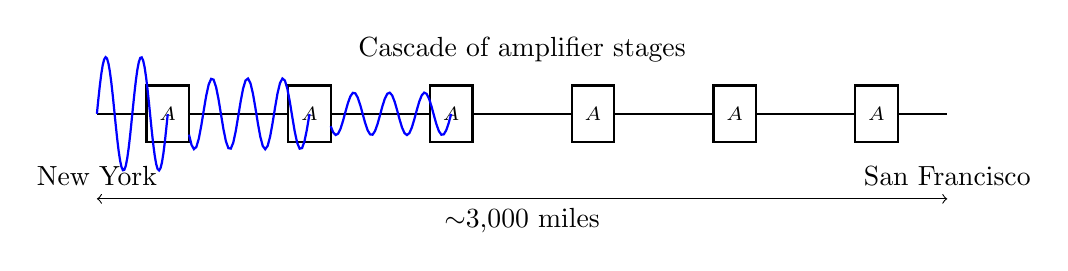
\begin{tikzpicture}[scale=0.9]
    % Telephone line representation
    \draw[thick] (0,0) -- (12,0);

    % Amplifier stages
    \foreach \x in {1,3,5,7,9,11} {
        \draw[thick,fill=white] (\x-0.3,-0.4) rectangle (\x+0.3,0.4);
        \node at (\x,0) {\scriptsize $A$};
    }

    % Signal attenuation representation
    \draw[blue,thick,domain=0:1,samples=50] plot (\x, {0.8*sin(720*\x)});
    \draw[blue,thick,domain=1.3:3,samples=50] plot (\x, {0.5*sin(720*\x)});
    \draw[blue,thick,domain=3.3:5,samples=50] plot (\x, {0.3*sin(720*\x)});

    % Labels
    \node[below] at (0,-0.6) {New York};
    \node[below] at (12,-0.6) {San Francisco};
    \node[above] at (6,0.6) {Cascade of amplifier stages};

    % Distance markers
    \draw[<->] (0,-1.2) -- (12,-1.2);
    \node[below] at (6,-1.2) {$\sim$3,000 miles};
\end{tikzpicture}
\caption{Transcontinental telephone transmission required cascaded amplifier stages to compensate for line attenuation. Each stage contributed frequency-dependent gain and phase characteristics.}
\label{fig:cascade_amplifiers}
\end{figure}

The mathematical challenge was formidable. Analyzing the stability of even a single feedback amplifier required solving high-order differential equations. With multiple amplifiers, the mathematics became intractable using classical methods.

\subsection{Hendrik Bode and the Logarithmic Revolution}

\textbf{Hendrik Wade Bode} (1905--1982), a Dutch-American engineer at Bell Labs, developed an elegant solution to this complexity. His key insight was deceptively simple: \textit{plot system characteristics on logarithmic scales}.

\begin{historicalbox}
Bode joined Bell Labs in 1926 after earning his Ph.D. in physics from Columbia University at age 21. He spent his entire career at Bell Labs, eventually becoming Director of Mathematical Research. His 1945 book \textit{Network Analysis and Feedback Amplifier Design} remains a classic reference.
\end{historicalbox}

Consider $N$ amplifiers connected in cascade, each with transfer function $G_i(s)$. The overall transfer function is the product:
\begin{equation}
G_{\text{total}}(s) = G_1(s) \cdot G_2(s) \cdot \ldots \cdot G_N(s) = \prod_{i=1}^{N} G_i(s)
\label{eq:cascade_product}
\end{equation}

At sinusoidal steady state with $s = \jw$, the magnitude and phase are:
\begin{align}
\magn{G_{\text{total}}(\jw)} &= \prod_{i=1}^{N} \magn{G_i(\jw)} \label{eq:mag_product}\\
\phase{G_{\text{total}}(\jw)} &= \sum_{i=1}^{N} \phase{G_i(\jw)} \label{eq:phase_sum}
\end{align}

Bode's stroke of genius was to express magnitude in \textit{decibels}:
\begin{equation}
\boxed{\magn{G}_{\text{dB}} = 20 \log_{10} \magn{G(\jw)}}
\label{eq:decibel_def}
\end{equation}

Taking the logarithm of \cref{eq:mag_product}:
\begin{equation}
\magn{G_{\text{total}}}_{\text{dB}} = \sum_{i=1}^{N} \magn{G_i}_{\text{dB}}
\label{eq:db_sum}
\end{equation}

\begin{keypoint}
In decibels, cascaded system gains \textbf{add} rather than multiply. This transforms the analysis of complex systems into simple graphical addition---a task easily performed by hand or, in Bode's era, with a slide rule.
\end{keypoint}

The decibel, originally defined for power ratios in telephony (one-tenth of a \textit{bel}, named after Alexander Graham Bell), proved ideal for this application. When using decibels, multiplication becomes addition, making cascaded system analysis a matter of simple superposition. Furthermore, the logarithmic scale compresses very large and very small numbers into manageable ranges, while asymptotic behavior conveniently appears as straight lines on log-log plots.

\subsection{Harry Nyquist and the Stability Criterion}

While Bode developed graphical methods for analyzing system characteristics, his colleague \textbf{Harry Nyquist} (1889--1976) addressed the fundamental question of stability.

\begin{historicalbox}
Harry Nyquist, a Swedish-American engineer, made foundational contributions to both control theory and information theory. His 1932 paper ``Regeneration Theory'' established the theoretical basis for analyzing feedback amplifier stability using frequency response data.
\end{historicalbox}

Before Nyquist, determining stability required finding the roots of the characteristic polynomial---a task that becomes extremely difficult for systems of order higher than four. Nyquist showed that stability could be determined entirely from the frequency response, without solving any polynomial equations.

The \textbf{Nyquist stability criterion} relates the number of encirclements of the critical point $(-1, 0)$ in the complex plane to the number of closed-loop poles in the right half-plane. This graphical criterion, when combined with Bode's logarithmic plots, provided engineers with practical tools for designing stable high-gain amplifiers.

\subsection{The Fundamental Insight: Sinusoids as Eigenfunctions}

The theoretical foundation for frequency response methods rests on a remarkable mathematical property: \textit{sinusoidal signals are eigenfunctions of linear time-invariant (LTI) systems}.

\begin{theorem}[Eigenfunction Property of LTI Systems]
\label{thm:eigenfunction}
If a sinusoidal input $x(t) = A\sin(\omega t + \phi)$ is applied to a stable LTI system with transfer function $G(s)$, then after transients decay, the steady-state output is also sinusoidal at the same frequency:
\begin{equation}
y_{ss}(t) = A\magn{G(\jw)}\sin\left(\omega t + \phi + \phase{G(\jw)}\right)
\label{eq:sinusoidal_ss}
\end{equation}
\end{theorem}

\begin{proof}
Consider the input $x(t) = Ae^{j\omega t}$ (using complex exponential notation). For an LTI system with impulse response $h(t)$, the output is the convolution:
\begin{align}
y(t) &= \int_{-\infty}^{\infty} h(\tau) x(t-\tau) \, d\tau = \int_{-\infty}^{\infty} h(\tau) Ae^{j\omega(t-\tau)} \, d\tau \\
&= Ae^{j\omega t} \int_{-\infty}^{\infty} h(\tau) e^{-j\omega\tau} \, d\tau = Ae^{j\omega t} \cdot G(\jw)
\end{align}
where $G(\jw) = \mathcal{L}\{h(t)\}|_{s=\jw}$ is the frequency response. Since $G(\jw) = \magn{G(\jw)}e^{j\phase{G(\jw)}}$:
\begin{equation}
y(t) = A\magn{G(\jw)} e^{j(\omega t + \phase{G(\jw)})}
\end{equation}
Taking the imaginary part recovers the result for $\sin(\omega t)$ input.
\end{proof}

This property is profound: to characterize how a system responds to \textit{any} input, we need only measure its response to sinusoids across the frequency spectrum. This is because any reasonable input signal can be decomposed into sinusoidal components via Fourier analysis.

%=============================================================================
\section{Modern Applications}
\label{sec:modern_apps}
%=============================================================================

The frequency response methods pioneered for telephone amplifiers have found application across virtually every domain of engineering. The underlying principle---that system behavior can be characterized by its response to sinusoidal inputs---remains as powerful today as it was in Bode's time.

\subsection{Audio System Design}

In audio engineering, frequency response is the fundamental specification. Equalizers, whether hardware or software, operate directly in the frequency domain. Graphic equalizers adjust gain in discrete frequency bands, while parametric equalizers provide more flexible control by allowing adjustment of center frequency, bandwidth, and gain simultaneously. Crossover networks serve a different purpose entirely, dividing audio signals among different drivers such as woofers and tweeters to ensure each component reproduces only the frequencies it handles best.

The human ear's frequency response (approximately 20 Hz to 20 kHz) defines the relevant analysis range. Audio specifications invariably include frequency response plots, typically requiring $\pm 3\dB$ flatness over the audible range.

\subsection{Filter Design}

Frequency response analysis is essential for designing analog and digital filters. Anti-aliasing filters, required before analog-to-digital conversion to satisfy the Nyquist criterion, must provide sufficient attenuation above the Nyquist frequency---typically 60--80 dB, a specification read directly from the Bode magnitude plot. In industrial environments containing electromagnetic interference at specific frequencies such as 60 Hz power line noise or switching power supply harmonics, notch filters designed using Bode techniques effectively remove these disturbances. Communication systems similarly rely on precise frequency-domain specifications for channel selection, pulse shaping, and equalization.

\subsection{Control Loop Bandwidth Specification}

In modern control system design, performance is often specified in terms of frequency-domain metrics. The bandwidth, defined as the frequency at which the closed-loop magnitude drops to $-3\dB$ of its low-frequency value, directly correlates with response speed---higher bandwidth implies faster response. Stability margins, including gain margin and phase margin (detailed in \cref{sec:stability_margins}), quantify robustness to modeling errors and component variations. The sensitivity function $S(\jw) = 1/(1+G(\jw)H(\jw))$ characterizes disturbance rejection capability across the frequency spectrum.

\subsection{Electromagnetic Compatibility (EMC)}

Regulatory compliance for electronic products requires frequency-domain analysis. Emissions testing verifies that products do not radiate electromagnetic energy above specified limits across frequency bands, as mandated by regulations such as FCC Part 15 and CISPR 22. Susceptibility testing ensures products operate correctly when exposed to electromagnetic fields at various frequencies. Power supply design presents particular challenges, as switching converters must attenuate high-frequency noise sufficiently to meet conducted emissions limits.

The Bode plot provides a natural framework for specifying and verifying filter performance in EMC applications.

%=============================================================================
\section{Mathematical Foundation}
\label{sec:math_foundation}
%=============================================================================

\subsection{Frequency Response Function}

For a system with transfer function $G(s)$, the \textbf{frequency response} is obtained by evaluating along the imaginary axis:
\begin{equation}
G(\jw) = G(s)\big|_{s=\jw}
\label{eq:freq_response}
\end{equation}

This complex-valued function can be expressed in polar form:
\begin{equation}
\boxed{G(\jw) = \magn{G(\jw)} e^{j\phase{G(\jw)}}}
\label{eq:polar_form}
\end{equation}

where $\magn{G(\jw)}$ denotes the \textbf{magnitude} (gain) at frequency $\omega$, and $\phase{G(\jw)}$ denotes the \textbf{phase} (angle) at frequency $\omega$.

Equivalently, in rectangular form:
\begin{equation}
G(\jw) = \text{Re}\{G(\jw)\} + j\,\text{Im}\{G(\jw)\}
\label{eq:rectangular}
\end{equation}

with:
\begin{align}
\magn{G(\jw)} &= \sqrt{\text{Re}^2\{G(\jw)\} + \text{Im}^2\{G(\jw)\}} \\
\phase{G(\jw)} &= \arctan\left(\frac{\text{Im}\{G(\jw)\}}{\text{Re}\{G(\jw)\}}\right)
\end{align}

\subsection{Bode Plot Construction}

A \textbf{Bode plot} consists of two graphs plotted against frequency on a logarithmic scale. The magnitude plot displays $20\log_{10}\magn{G(\jw)}$ in decibels (dB) versus $\log_{10}\omega$, while the phase plot displays $\phase{G(\jw)}$ in degrees versus $\log_{10}\omega$.

\begin{keypoint}
The logarithmic frequency scale allows visualization of many decades of frequency on a single plot. The decibel scale for magnitude enables addition of cascaded elements. Together, these choices transform multiplicative transfer function factors into additive graphical contributions.
\end{keypoint}

\begin{figure}[htbp]
\centering
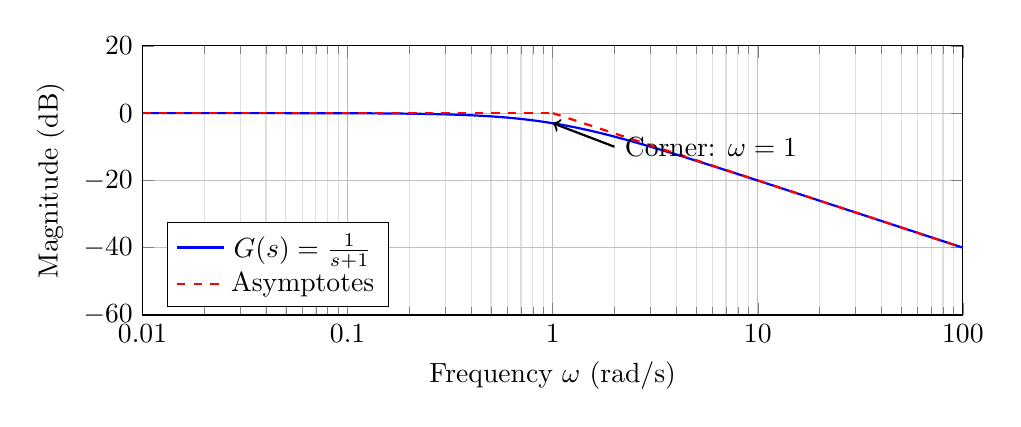
\begin{tikzpicture}
    \begin{semilogxaxis}[
        width=12cm, height=5cm,
        xlabel={Frequency $\omega$ (rad/s)},
        ylabel={Magnitude (dB)},
        xmin=0.01, xmax=100,
        ymin=-60, ymax=20,
        grid=both,
        minor grid style={gray!25},
        major grid style={gray!50},
        xtick={0.01,0.1,1,10,100},
        xticklabels={$0.01$,$0.1$,$1$,$10$,$100$},
        ytick={-60,-40,-20,0,20},
        legend pos=south west
    ]
    % Example magnitude response
    \addplot[blue,thick,domain=0.01:100,samples=200]
        {20*log10(1/sqrt(1+x^2))};
    \addlegendentry{$G(s) = \frac{1}{s+1}$}

    % Asymptotes
    \addplot[red,dashed,thick] coordinates {(0.01,0) (1,0)};
    \addplot[red,dashed,thick,domain=1:100,samples=50]
        {-20*log10(x)};
    \addlegendentry{Asymptotes}

    % Corner frequency marker
    \draw[<-,thick] (axis cs:1,-3) -- (axis cs:2,-10)
        node[right] {Corner: $\omega = 1$};
    \end{semilogxaxis}
\end{tikzpicture}

\vspace{0.5cm}

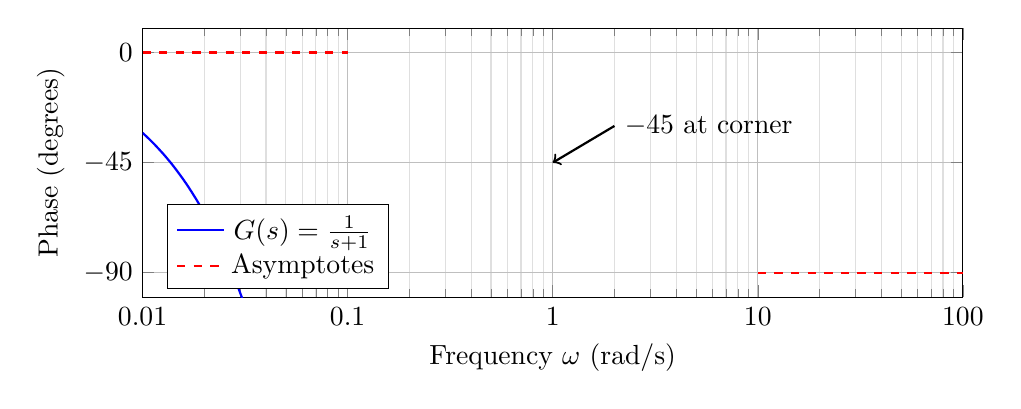
\begin{tikzpicture}
    \begin{semilogxaxis}[
        width=12cm, height=5cm,
        xlabel={Frequency $\omega$ (rad/s)},
        ylabel={Phase (degrees)},
        xmin=0.01, xmax=100,
        ymin=-100, ymax=10,
        grid=both,
        minor grid style={gray!25},
        major grid style={gray!50},
        xtick={0.01,0.1,1,10,100},
        xticklabels={$0.01$,$0.1$,$1$,$10$,$100$},
        ytick={-90,-45,0},
        legend pos=south west
    ]
    % Phase response
    \addplot[blue,thick,domain=0.01:100,samples=200]
        {-atan(x)*180/pi};
    \addlegendentry{$G(s) = \frac{1}{s+1}$}

    % Asymptotes
    \addplot[red,dashed,thick] coordinates {(0.01,0) (0.1,0)};
    \addplot[red,dashed,thick] coordinates {(10,-90) (100,-90)};
    \addlegendentry{Asymptotes}

    % -45 degree marker
    \draw[<-,thick] (axis cs:1,-45) -- (axis cs:2,-30)
        node[right] {$-45\degrees$ at corner};
    \end{semilogxaxis}
\end{tikzpicture}
\caption{Bode plot template showing magnitude (top) and phase (bottom) for a first-order system $G(s) = 1/(s+1)$. Asymptotes are shown as dashed red lines.}
\label{fig:bode_template}
\end{figure}

\subsection{First-Order System: $G(s) = \frac{1}{\tau s + 1}$}

Consider the first-order low-pass system with time constant $\tau$:
\begin{equation}
G(s) = \frac{1}{\tau s + 1}
\label{eq:first_order}
\end{equation}

Substituting $s = \jw$:
\begin{equation}
G(\jw) = \frac{1}{j\omega\tau + 1} = \frac{1}{1 + j\omega\tau}
\label{eq:first_order_jw}
\end{equation}

\textbf{Magnitude:}
\begin{equation}
\magn{G(\jw)} = \frac{1}{\sqrt{1 + (\omega\tau)^2}}
\label{eq:first_order_mag}
\end{equation}

In decibels:
\begin{equation}
\magn{G(\jw)}_{\text{dB}} = -20\log_{10}\sqrt{1 + (\omega\tau)^2} = -10\log_{10}\left(1 + \omega^2\tau^2\right)
\label{eq:first_order_db}
\end{equation}

\textbf{Phase:}
\begin{equation}
\phase{G(\jw)} = -\arctan(\omega\tau)
\label{eq:first_order_phase}
\end{equation}

\subsubsection{Asymptotic Analysis}

The power of Bode plots lies in their asymptotic approximations:

\textbf{Low frequency} ($\omega \ll 1/\tau$):
\begin{align}
\magn{G(\jw)}_{\text{dB}} &\approx -10\log_{10}(1) = 0\dB \\
\phase{G(\jw)} &\approx -\arctan(0) = 0\degrees
\end{align}

\textbf{High frequency} ($\omega \gg 1/\tau$):
\begin{align}
\magn{G(\jw)}_{\text{dB}} &\approx -10\log_{10}(\omega^2\tau^2) = -20\log_{10}(\omega\tau) \\
\phase{G(\jw)} &\approx -\arctan(\infty) = -90\degrees
\end{align}

The high-frequency asymptote has a slope of $-20\dB$ per decade (i.e., for every factor of 10 increase in frequency, the magnitude decreases by $20\dB$).

\textbf{Corner frequency} ($\omega = 1/\tau$):
\begin{align}
\magn{G(\jw)}_{\text{dB}} &= -10\log_{10}(2) \approx -3\dB \\
\phase{G(\jw)} &= -\arctan(1) = -45\degrees
\end{align}

\begin{definition}[Corner Frequency]
The \textbf{corner frequency} (or break frequency) $\omega_c = 1/\tau$ is the frequency at which the low-frequency and high-frequency asymptotes intersect. At the corner frequency, the actual magnitude is $3\dB$ below the asymptotic value, and the phase is $-45\degrees$ for a single real pole.
\end{definition}

\begin{figure}[htbp]
\centering
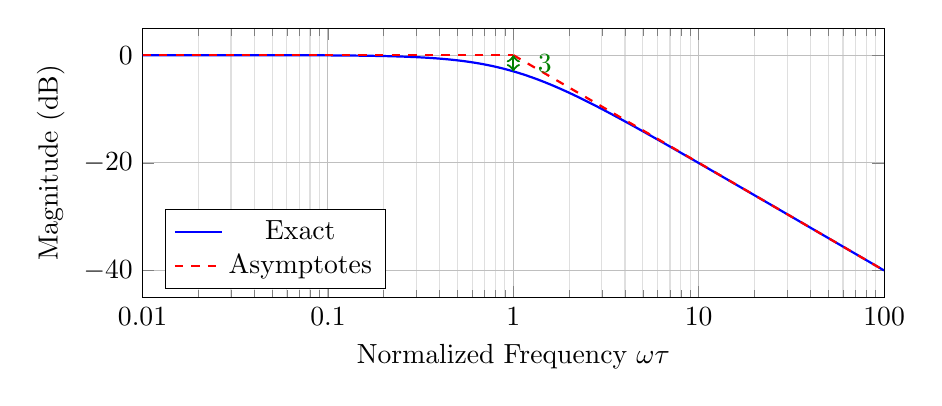
\begin{tikzpicture}
    \begin{semilogxaxis}[
        width=11cm, height=5cm,
        xlabel={Normalized Frequency $\omega\tau$},
        ylabel={Magnitude (dB)},
        xmin=0.01, xmax=100,
        ymin=-45, ymax=5,
        grid=both,
        minor grid style={gray!25},
        major grid style={gray!50},
        xtick={0.01,0.1,1,10,100},
        xticklabels={$0.01$,$0.1$,$1$,$10$,$100$},
        legend pos=south west
    ]
    % Exact response
    \addplot[blue,thick,domain=0.01:100,samples=200]
        {-10*log10(1+x^2)};
    \addlegendentry{Exact}

    % Low frequency asymptote
    \addplot[red,dashed,thick] coordinates {(0.01,0) (1,0)};

    % High frequency asymptote
    \addplot[red,dashed,thick,domain=1:100,samples=50]
        {-20*log10(x)};
    \addlegendentry{Asymptotes}

    % Error annotation
    \draw[<->,thick,green!50!black] (axis cs:1,0) -- (axis cs:1,-3);
    \node[right,green!50!black] at (axis cs:1.2,-1.5) {$3\dB$};
    \end{semilogxaxis}
\end{tikzpicture}

\vspace{0.3cm}

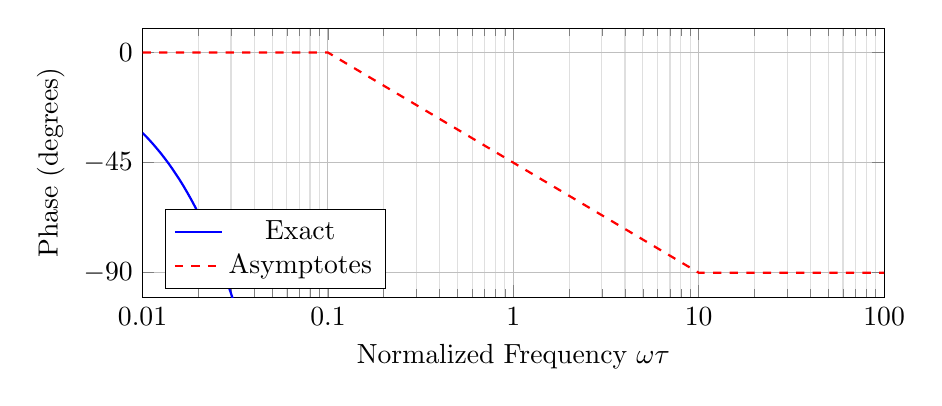
\begin{tikzpicture}
    \begin{semilogxaxis}[
        width=11cm, height=5cm,
        xlabel={Normalized Frequency $\omega\tau$},
        ylabel={Phase (degrees)},
        xmin=0.01, xmax=100,
        ymin=-100, ymax=10,
        grid=both,
        minor grid style={gray!25},
        major grid style={gray!50},
        xtick={0.01,0.1,1,10,100},
        xticklabels={$0.01$,$0.1$,$1$,$10$,$100$},
        ytick={-90,-45,0},
        legend pos=south west
    ]
    % Exact phase
    \addplot[blue,thick,domain=0.01:100,samples=200]
        {-atan(x)*180/pi};
    \addlegendentry{Exact}

    % Asymptotic approximation
    \addplot[red,dashed,thick] coordinates {(0.01,0) (0.1,0) (10,-90) (100,-90)};
    \addlegendentry{Asymptotes}
    \end{semilogxaxis}
\end{tikzpicture}
\caption{First-order low-pass system Bode plot. The asymptotic approximation (dashed) is within $3\dB$ of the exact response (solid) at the corner frequency.}
\label{fig:first_order_bode}
\end{figure}

\subsection{Second-Order System}

Consider the standard second-order system:
\begin{equation}
G(s) = \frac{\omega_n^2}{s^2 + 2\zeta\omega_n s + \omega_n^2}
\label{eq:second_order}
\end{equation}

where $\omega_n$ is the natural frequency and $\zeta$ is the damping ratio.

Substituting $s = \jw$:
\begin{equation}
G(\jw) = \frac{\omega_n^2}{\omega_n^2 - \omega^2 + 2j\zeta\omega_n\omega}
\label{eq:second_order_jw}
\end{equation}

Let $u = \omega/\omega_n$ (normalized frequency):
\begin{equation}
G(ju\omega_n) = \frac{1}{1 - u^2 + 2j\zeta u}
\label{eq:second_order_normalized}
\end{equation}

\textbf{Magnitude:}
\begin{equation}
\magn{G(\jw)} = \frac{1}{\sqrt{(1-u^2)^2 + (2\zeta u)^2}}
\label{eq:second_order_mag}
\end{equation}

\textbf{Phase:}
\begin{equation}
\phase{G(\jw)} = -\arctan\left(\frac{2\zeta u}{1 - u^2}\right)
\label{eq:second_order_phase}
\end{equation}

\subsubsection{Asymptotic Behavior}

\textbf{Low frequency} ($\omega \ll \omega_n$, $u \ll 1$):
\begin{align}
\magn{G}_{\text{dB}} &\approx 0\dB \\
\phase{G} &\approx 0\degrees
\end{align}

\textbf{High frequency} ($\omega \gg \omega_n$, $u \gg 1$):
\begin{align}
\magn{G}_{\text{dB}} &\approx -40\log_{10}u = -40\log_{10}(\omega/\omega_n) \\
\phase{G} &\approx -180\degrees
\end{align}

The high-frequency asymptote has a slope of $-40\dB$/decade (compared to $-20\dB$/decade for first-order systems).

\subsubsection{Resonant Peak}

For underdamped systems ($\zeta < 1/\sqrt{2} \approx 0.707$), the magnitude exhibits a resonant peak. The peak occurs at:
\begin{equation}
\omega_r = \omega_n\sqrt{1 - 2\zeta^2} \quad \text{(for } \zeta < 0.707\text{)}
\label{eq:resonant_freq}
\end{equation}

The peak magnitude is:
\begin{equation}
M_r = \frac{1}{2\zeta\sqrt{1 - \zeta^2}} \quad \text{or} \quad M_{r,\text{dB}} = -20\log_{10}(2\zeta\sqrt{1-\zeta^2})
\label{eq:resonant_peak}
\end{equation}

\begin{figure}[htbp]
\centering
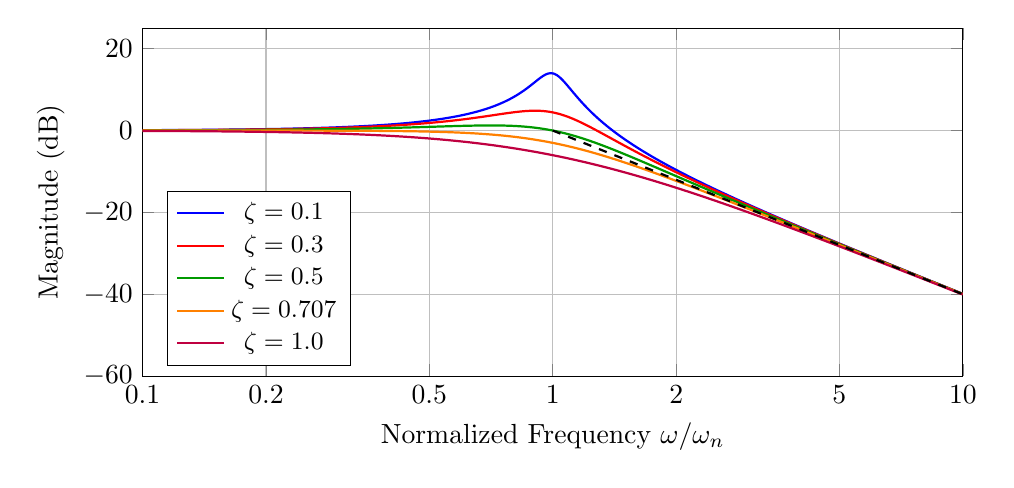
\begin{tikzpicture}
    \begin{semilogxaxis}[
        width=12cm, height=6cm,
        xlabel={Normalized Frequency $\omega/\omega_n$},
        ylabel={Magnitude (dB)},
        xmin=0.1, xmax=10,
        ymin=-60, ymax=25,
        grid=both,
        minor grid style={gray!25},
        major grid style={gray!50},
        xtick={0.1,0.2,0.5,1,2,5,10},
        xticklabels={$0.1$,$0.2$,$0.5$,$1$,$2$,$5$,$10$},
        legend pos=south west,
        legend style={font=\small}
    ]
    % Different damping ratios
    \addplot[blue,thick,domain=0.1:10,samples=300]
        {20*log10(1/sqrt((1-x^2)^2 + (2*0.1*x)^2))};
    \addlegendentry{$\zeta = 0.1$}

    \addplot[red,thick,domain=0.1:10,samples=300]
        {20*log10(1/sqrt((1-x^2)^2 + (2*0.3*x)^2))};
    \addlegendentry{$\zeta = 0.3$}

    \addplot[green!60!black,thick,domain=0.1:10,samples=300]
        {20*log10(1/sqrt((1-x^2)^2 + (2*0.5*x)^2))};
    \addlegendentry{$\zeta = 0.5$}

    \addplot[orange,thick,domain=0.1:10,samples=300]
        {20*log10(1/sqrt((1-x^2)^2 + (2*0.707*x)^2))};
    \addlegendentry{$\zeta = 0.707$}

    \addplot[purple,thick,domain=0.1:10,samples=300]
        {20*log10(1/sqrt((1-x^2)^2 + (2*1.0*x)^2))};
    \addlegendentry{$\zeta = 1.0$}

    % Asymptote
    \addplot[black,dashed,thick,domain=1:10,samples=50]
        {-40*log10(x)};
    \end{semilogxaxis}
\end{tikzpicture}

\vspace{0.3cm}

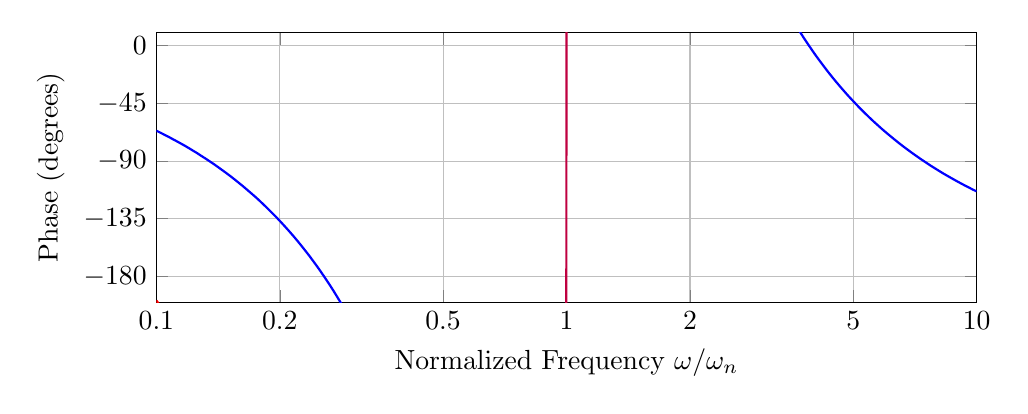
\begin{tikzpicture}
    \begin{semilogxaxis}[
        width=12cm, height=5cm,
        xlabel={Normalized Frequency $\omega/\omega_n$},
        ylabel={Phase (degrees)},
        xmin=0.1, xmax=10,
        ymin=-200, ymax=10,
        grid=both,
        minor grid style={gray!25},
        major grid style={gray!50},
        xtick={0.1,0.2,0.5,1,2,5,10},
        xticklabels={$0.1$,$0.2$,$0.5$,$1$,$2$,$5$,$10$},
        ytick={-180,-135,-90,-45,0},
        legend pos=south west,
        legend style={font=\small}
    ]
    % Different damping ratios - phase
    \addplot[blue,thick,domain=0.1:0.99,samples=100]
        {-atan(2*0.1*x/(1-x^2))*180/pi};
    \addplot[blue,thick,domain=1.01:10,samples=100]
        {-180-atan(2*0.1*x/(1-x^2))*180/pi};

    \addplot[red,thick,domain=0.1:0.99,samples=100]
        {-atan(2*0.3*x/(1-x^2))*180/pi};
    \addplot[red,thick,domain=1.01:10,samples=100]
        {-180-atan(2*0.3*x/(1-x^2))*180/pi};

    \addplot[green!60!black,thick,domain=0.1:0.99,samples=100]
        {-atan(2*0.5*x/(1-x^2))*180/pi};
    \addplot[green!60!black,thick,domain=1.01:10,samples=100]
        {-180-atan(2*0.5*x/(1-x^2))*180/pi};

    \addplot[orange,thick,domain=0.1:0.99,samples=100]
        {-atan(2*0.707*x/(1-x^2))*180/pi};
    \addplot[orange,thick,domain=1.01:10,samples=100]
        {-180-atan(2*0.707*x/(1-x^2))*180/pi};

    \addplot[purple,thick,domain=0.1:10,samples=200]
        {-atan(2*1.0*x/(1-x^2))*180/pi - (x>1 ? 180 : 0)};
    \end{semilogxaxis}
\end{tikzpicture}
\caption{Second-order system Bode plots for various damping ratios $\zeta$. Note the resonant peak for $\zeta < 0.707$ and the phase transition through $-90\degrees$ at $\omega = \omega_n$.}
\label{fig:second_order_bode}
\end{figure}

\subsection{Combining Elements: Poles and Zeros}

A general transfer function can be factored as:
\begin{equation}
G(s) = K \frac{\prod_{i=1}^{m}(s - z_i)}{\prod_{j=1}^{n}(s - p_j)}
\label{eq:general_tf}
\end{equation}

where $z_i$ are zeros and $p_j$ are poles.

For Bode plot construction, we express this in \textit{time constant form}:
\begin{equation}
G(s) = K_0 \frac{\prod_{i}(1 + \tau_{z_i}s)}{\prod_{j}(1 + \tau_{p_j}s)}
\label{eq:time_constant_form}
\end{equation}

where $K_0$ is the DC gain (for a type-0 system).

\begin{keypoint}
\textbf{Bode Plot Construction Rules:}

\begin{center}
\begin{tabular}{p{3.5cm}p{3cm}p{3cm}p{3.5cm}}
\toprule
\textbf{Element} & \textbf{Break Frequency} & \textbf{Magnitude Effect} & \textbf{Phase Effect} \\
\midrule
Gain $K_0$ & None & $+20\log_{10}|K_0|$ dB offset & $0\degrees$ (or $180\degrees$ if $K_0 < 0$) \\
Pole at origin ($1/s$) & All frequencies & $-20$ dB/decade & $-90\degrees$ \\
Zero at origin ($s$) & All frequencies & $+20$ dB/decade & $+90\degrees$ \\
Real pole $\frac{1}{1+\tau s}$ & $\omega = 1/\tau$ & Adds $-20$ dB/decade & Adds $-90\degrees$ \\
Real zero $(1+\tau s)$ & $\omega = 1/\tau$ & Adds $+20$ dB/decade & Adds $+90\degrees$ \\
Complex poles & $\omega = \omega_n$ & Adds $-40$ dB/decade; possible resonant peak & Adds $-180\degrees$ \\
Complex zeros & $\omega = \omega_n$ & Adds $+40$ dB/decade & Adds $+180\degrees$ \\
\bottomrule
\end{tabular}
\end{center}
\end{keypoint}

\begin{examplebox}[Combining First-Order Terms]
\label{ex:combining}
Sketch the Bode plot for:
\begin{equation}
G(s) = \frac{10(s+1)}{s(s+10)}
\end{equation}

\textbf{Solution:} Rewrite in standard form:
\begin{equation}
G(s) = \frac{10 \cdot 1 \cdot (1 + s)}{s \cdot 10 \cdot (1 + s/10)} = \frac{1 + s}{s(1 + s/10)}
\end{equation}

The transfer function contains the following components: a DC gain of $K_0 = 1$ ($0\dB$ at $\omega = 1$), a pole at the origin ($1/s$), a zero at $\omega = 1$ from the term $(1 + s)$, and a pole at $\omega = 10$ from the term $1/(1 + s/10)$.

Starting from low frequency and tracing the asymptotic magnitude, the slope is $-20\dB$/decade for $\omega < 1$ due to the pole at origin. At $\omega = 1$, the zero contributes $+20\dB$/decade, bringing the net slope to $0\dB$/decade. Finally, at $\omega = 10$, the pole adds $-20\dB$/decade, returning the net slope to $-20\dB$/decade.
\end{examplebox}

\subsection{Stability Margins}
\label{sec:stability_margins}

For a unity feedback system with open-loop transfer function $G(s)$, the closed-loop stability can be assessed directly from the open-loop Bode plot.

\begin{figure}[htbp]
\centering
\begin{tikzpicture}[auto, node distance=2cm, >=Stealth]
    % Blocks
    \node[draw, circle, minimum size=0.6cm] (sum) {};
    \node[draw, minimum width=1.5cm, minimum height=1cm, right=1.5cm of sum] (G) {$G(s)$};

    % Connections
    \draw[->] ($(sum.west)+(-1.5,0)$) -- node[pos=0.3,above] {$R(s)$} (sum.west);
    \draw[->] (sum.east) -- (G.west);
    \draw[->] (G.east) -- node[pos=0.5,above] {$Y(s)$} ($(G.east)+(1.5,0)$);
    \draw[->] ($(G.east)+(1,0)$) -- ++(0,-1) -| (sum.south);

    % Sum labels
    \node at ($(sum.north west)+(0.15,0.1)$) {\tiny $+$};
    \node at ($(sum.south)+(0.15,-0.1)$) {\tiny $-$};
\end{tikzpicture}
\caption{Unity feedback configuration. The closed-loop transfer function is $T(s) = G(s)/(1+G(s))$.}
\label{fig:unity_feedback}
\end{figure}

The closed-loop characteristic equation is $1 + G(s) = 0$, or $G(s) = -1$.

In polar form, instability occurs when:
\begin{equation}
\magn{G(\jw)} = 1 \quad \text{and} \quad \phase{G(\jw)} = -180\degrees
\label{eq:instability_condition}
\end{equation}

\begin{definition}[Gain Crossover Frequency]
The \textbf{gain crossover frequency} $\omega_{gc}$ is the frequency at which $\magn{G(\jw_{gc})} = 1$ (i.e., $0\dB$).
\end{definition}

\begin{definition}[Phase Crossover Frequency]
The \textbf{phase crossover frequency} $\omega_{pc}$ is the frequency at which $\phase{G(\jw_{pc})} = -180\degrees$.
\end{definition}

\begin{definition}[Gain Margin]
The \textbf{gain margin} (GM) is the factor by which the open-loop gain can be increased before the system becomes unstable:
\begin{equation}
\text{GM} = \frac{1}{\magn{G(\jw_{pc})}} \quad \text{or} \quad \text{GM}_{\text{dB}} = -20\log_{10}\magn{G(\jw_{pc})}
\label{eq:gain_margin}
\end{equation}
\end{definition}

\begin{definition}[Phase Margin]
The \textbf{phase margin} (PM) is the additional phase lag that would bring the system to the verge of instability:
\begin{equation}
\text{PM} = 180\degrees + \phase{G(\jw_{gc})}
\label{eq:phase_margin}
\end{equation}
\end{definition}

\begin{figure}[htbp]
\centering
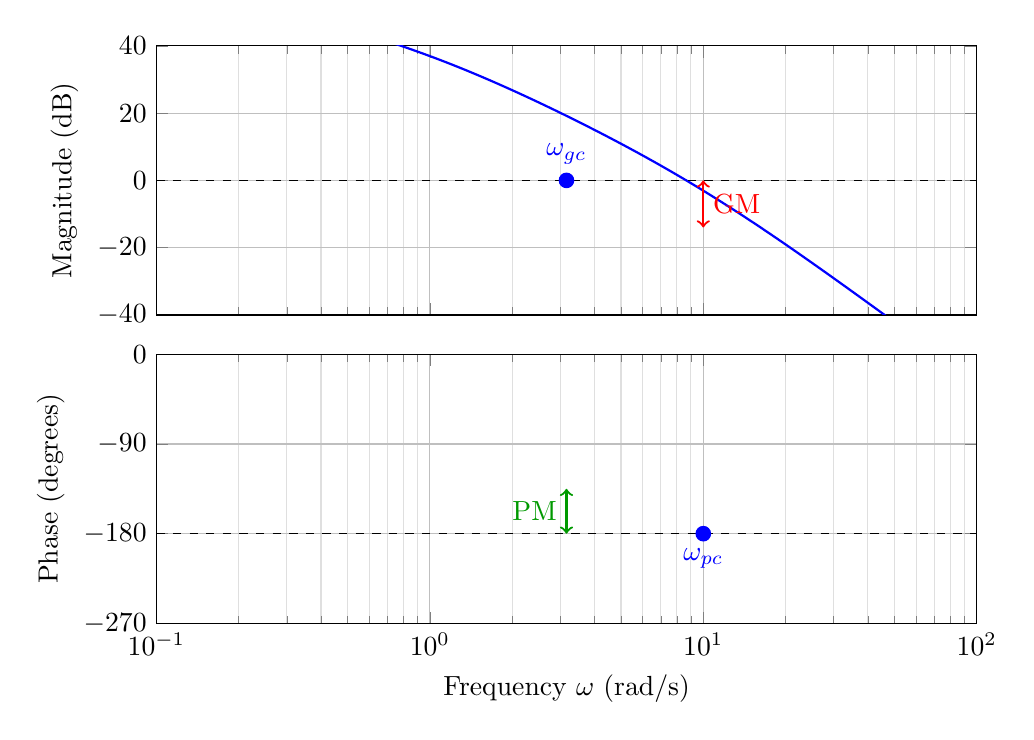
\begin{tikzpicture}
    \begin{semilogxaxis}[
        name=mag,
        width=12cm, height=5cm,
        ylabel={Magnitude (dB)},
        xmin=0.1, xmax=100,
        ymin=-40, ymax=40,
        grid=both,
        minor grid style={gray!25},
        major grid style={gray!50},
        xtick={0.1,1,10,100},
        xticklabels={},
        ytick={-40,-20,0,20,40}
    ]
    % Open-loop magnitude
    \addplot[blue,thick,domain=0.1:100,samples=200]
        {20*log10(100/(x*sqrt(1+x^2)*sqrt(1+(x/10)^2)))};

    % 0 dB line
    \addplot[black,dashed] coordinates {(0.1,0) (100,0)};

    % Gain crossover
    \draw[red,thick,<->] (axis cs:10,0) -- (axis cs:10,-14);
    \node[red,right] at (axis cs:10,-7) {GM};

    % Markers
    \node[blue,circle,fill,inner sep=2pt] at (axis cs:3.16,0) {};
    \node[above,blue] at (axis cs:3.16,2) {$\omega_{gc}$};
    \end{semilogxaxis}

    \begin{semilogxaxis}[
        at={(mag.south west)},
        anchor=north west,
        yshift=-0.5cm,
        width=12cm, height=5cm,
        xlabel={Frequency $\omega$ (rad/s)},
        ylabel={Phase (degrees)},
        xmin=0.1, xmax=100,
        ymin=-270, ymax=0,
        grid=both,
        minor grid style={gray!25},
        major grid style={gray!50},
        xtick={0.1,1,10,100},
        ytick={-270,-180,-90,0}
    ]
    % Open-loop phase
    \addplot[blue,thick,domain=0.1:100,samples=200]
        {-90 - atan(x)*180/pi - atan(x/10)*180/pi};

    % -180 degree line
    \addplot[black,dashed] coordinates {(0.1,-180) (100,-180)};

    % Phase margin
    \draw[green!60!black,thick,<->] (axis cs:3.16,-135) -- (axis cs:3.16,-180);
    \node[green!60!black,left] at (axis cs:3.16,-157) {PM};

    % Phase crossover
    \node[blue,circle,fill,inner sep=2pt] at (axis cs:10,-180) {};
    \node[below,blue] at (axis cs:10,-185) {$\omega_{pc}$};
    \end{semilogxaxis}
\end{tikzpicture}
\caption{Gain margin and phase margin illustrated on a Bode plot. GM is measured at the phase crossover frequency $\omega_{pc}$; PM is measured at the gain crossover frequency $\omega_{gc}$. Positive margins indicate stability.}
\label{fig:stability_margins}
\end{figure}

\begin{designtip}
Typical design specifications for robust control systems require a gain margin of at least $6\dB$ (a factor of 2) and a phase margin of at least $45\degrees$. These margins provide robustness against modeling uncertainties, component variations, and unmodeled dynamics.
\end{designtip}

%=============================================================================
\section{Laboratory Experiment: Frequency Response Measurement}
\label{sec:experiment}
%=============================================================================

\begin{experimentbox}
\textbf{Objective:} Measure the frequency response of an RC low-pass filter and compare with theoretical predictions.

\textbf{Equipment:} Arduino Uno or similar microcontroller, resistor ($R = 10\,\text{k}\Omega$), capacitor ($C = 100\,\text{nF}$ or 0.1 $\mu$F), oscilloscope (or second Arduino for data acquisition), breadboard, and connecting wires.
\end{experimentbox}

\subsection{Theoretical Background}

The RC low-pass filter has the transfer function:
\begin{equation}
G(s) = \frac{V_{out}(s)}{V_{in}(s)} = \frac{1}{RCs + 1} = \frac{1}{\tau s + 1}
\label{eq:rc_filter}
\end{equation}

where $\tau = RC$ is the time constant.

For $R = 10\,\text{k}\Omega$ and $C = 100\,\text{nF}$:
\begin{equation}
\tau = RC = 10 \times 10^3 \times 100 \times 10^{-9} = 1\,\text{ms}
\end{equation}

The corner frequency is:
\begin{equation}
f_c = \frac{1}{2\pi\tau} = \frac{1}{2\pi \times 0.001} \approx 159\,\text{Hz}
\end{equation}

\subsection{Circuit Construction}

\begin{figure}[htbp]
\centering
\begin{circuitikz}[scale=1.2]
    % Input
    \draw (0,0) node[ground]{} to[short] (0,2)
          to[R, l=$R$, a=10k$\Omega$] (3,2)
          to[short] (4,2);
    \draw (3,2) to[C, l_=$C$, a^=100nF] (3,0) node[ground]{};

    % Output labels
    \draw (4,2) to[short, -o] (5,2) node[right] {$V_{out}$};
    \draw (0,2) to[short, -o] (-1,2) node[left] {$V_{in}$};

    % Arduino connection labels
    \node[above] at (-0.5,2.3) {\scriptsize Arduino PWM};
    \node[above] at (4.5,2.3) {\scriptsize Arduino ADC};
\end{circuitikz}
\caption{RC low-pass filter circuit for frequency response measurement.}
\label{fig:rc_circuit}
\end{figure}

\subsection{Arduino Code for Sine Wave Generation}

The following algorithm generates sine wave outputs at various frequencies using PWM and measures the filter's response.

\begin{algorithm}
\caption{Frequency Response Measurement for RC Filter}
\begin{algorithmic}[1]
\State \textbf{Initialize:} Configure PWM output pin, ADC input pins, serial communication
\State \textbf{Define} test frequencies: $F \gets \{10, 20, 50, 100, 159, 200, 500, 1000, 2000, 5000\}$ Hz
\State Set PWM base frequency to approximately 31 kHz for better sine approximation
\State
\For{each frequency $f$ in $F$}
    \State $T \gets 1/f$ \Comment{Period in seconds}
    \State $N_{samples} \gets 100$
    \State $\Delta t \gets T / N_{samples}$
    \State Initialize accumulators: $\Sigma_{in}, \Sigma_{out}, \Sigma_{in}^2, \Sigma_{out}^2 \gets 0$
    \State
    \For{$cycle = 1$ to $10$}
        \For{$j = 0$ to $N_{samples} - 1$}
            \State $t \gets j \cdot \Delta t$
            \State $V_{PWM} \gets 127 + 127 \cdot \sin(2\pi f t)$ \Comment{Generate sine wave}
            \State Output $V_{PWM}$ to PWM pin
            \State Wait for duration $\Delta t$
            \State $V_{in} \gets$ Read ADC input (reference)
            \State $V_{out} \gets$ Read ADC output (filtered)
            \State Update accumulators: $\Sigma_{in} \mathrel{+}= V_{in}$, $\Sigma_{out} \mathrel{+}= V_{out}$
            \State Update squared accumulators: $\Sigma_{in}^2 \mathrel{+}= V_{in}^2$, $\Sigma_{out}^2 \mathrel{+}= V_{out}^2$
        \EndFor
    \EndFor
    \State
    \State $n \gets N_{samples} \times 10$
    \State $V_{in,RMS} \gets \sqrt{\Sigma_{in}^2/n - (\Sigma_{in}/n)^2}$ \Comment{Calculate RMS values}
    \State $V_{out,RMS} \gets \sqrt{\Sigma_{out}^2/n - (\Sigma_{out}/n)^2}$
    \State $|G| \gets V_{out,RMS} / V_{in,RMS}$ \Comment{Magnitude ratio}
    \State $\phi \gets -\arctan(f / f_c) \times 180/\pi$ \Comment{Phase estimate, $f_c = 159$ Hz}
    \State Output: frequency $f$, magnitude $|G|$, phase $\phi$
\EndFor
\end{algorithmic}
\end{algorithm}

\subsection{Data Collection and Analysis}

\begin{table}[htbp]
\centering
\caption{Expected vs.\ Measured Frequency Response}
\label{tab:freq_response}
\begin{tabular}{ccccc}
\toprule
Frequency & \multicolumn{2}{c}{Magnitude (ratio)} & \multicolumn{2}{c}{Phase (degrees)} \\
(Hz) & Theory & Measured & Theory & Measured \\
\midrule
10 & 0.998 & & $-3.6\degrees$ & \\
20 & 0.992 & & $-7.2\degrees$ & \\
50 & 0.954 & & $-17.4\degrees$ & \\
100 & 0.847 & & $-32.1\degrees$ & \\
159 & 0.707 & & $-45.0\degrees$ & \\
200 & 0.622 & & $-51.5\degrees$ & \\
500 & 0.303 & & $-72.3\degrees$ & \\
1000 & 0.157 & & $-81.0\degrees$ & \\
2000 & 0.079 & & $-85.5\degrees$ & \\
5000 & 0.032 & & $-88.2\degrees$ & \\
\bottomrule
\end{tabular}
\end{table}

\subsection{Plotting the Bode Diagram}

Students should plot their measured data alongside the theoretical curves:

\begin{equation}
\text{Magnitude (dB)} = 20\log_{10}\left(\frac{V_{out}}{V_{in}}\right)
\end{equation}

\begin{equation}
\text{Phase (degrees)} = -\arctan\left(\frac{f}{f_c}\right) \times \frac{180}{\pi}
\end{equation}

\subsection{Alternative Experiment: Motor Transfer Function}

For a more dynamic experiment, students can measure the frequency response of a DC motor. The procedure involves applying sinusoidal voltage commands at various frequencies while measuring the motor speed response using an encoder. From the collected data, the magnitude and phase are extracted at each test frequency. Finally, the measured frequency response data is fit to a first-order or second-order model to identify the system parameters.

The motor transfer function from voltage to speed typically has the form:
\begin{equation}
G(s) = \frac{K}{(\tau_e s + 1)(\tau_m s + 1)}
\end{equation}

where $\tau_e$ is the electrical time constant and $\tau_m$ is the mechanical time constant.

%=============================================================================
\section{Worked Examples}
\label{sec:examples}
%=============================================================================

\begin{example}[Sketching a First-Order Bode Plot]
\label{ex:first_order}
Sketch the Bode plot for $G(s) = \dfrac{100}{s + 10}$.

\textbf{Solution:}

\textit{Step 1: Convert to standard form.}
\begin{equation}
G(s) = \frac{100}{s + 10} = \frac{100}{10} \cdot \frac{1}{1 + s/10} = 10 \cdot \frac{1}{1 + s/10}
\end{equation}

\textit{Step 2: Identify components.}
The system has a DC gain of $K_0 = 10$, which corresponds to $20\log_{10}(10) = 20\dB$, and a first-order pole with corner frequency $\omega_c = 10$ rad/s.

\textit{Step 3: Construct magnitude plot.}
For frequencies $\omega < 10$ rad/s, the magnitude is constant at $20\dB$. At $\omega = 10$ rad/s, the rolloff begins at $-20\dB$/decade. For $\omega > 10$ rad/s, the slope continues at $-20\dB$/decade.

\textit{Step 4: Construct phase plot.}
For frequencies well below 10 rad/s, the phase is approximately $0\degrees$. At the corner frequency $\omega = 10$ rad/s, the phase equals $-45\degrees$. For frequencies well above 10 rad/s, the phase approaches $-90\degrees$.

\begin{center}
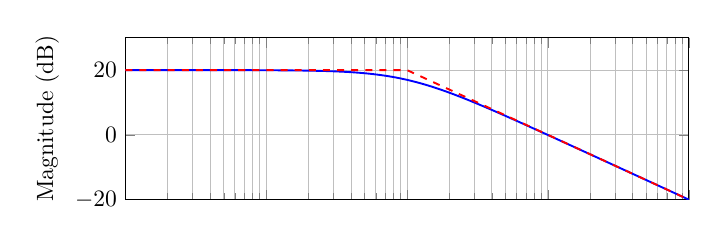
\begin{tikzpicture}[scale=0.85]
    \begin{semilogxaxis}[
        width=10cm, height=4cm,
        ylabel={Magnitude (dB)},
        xmin=0.1, xmax=1000,
        ymin=-20, ymax=30,
        grid=both,
        xtick={0.1,1,10,100,1000},
        xticklabels={},
        ytick={-20,0,20}
    ]
    \addplot[blue,thick,domain=0.1:1000,samples=200]
        {20 - 10*log10(1+(x/10)^2)};
    \addplot[red,dashed,thick] coordinates {(0.1,20) (10,20) (1000,-20)};
    \end{semilogxaxis}
\end{tikzpicture}

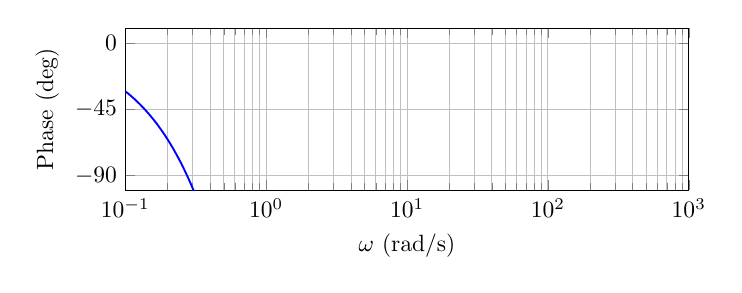
\begin{tikzpicture}[scale=0.85]
    \begin{semilogxaxis}[
        width=10cm, height=4cm,
        xlabel={$\omega$ (rad/s)},
        ylabel={Phase (deg)},
        xmin=0.1, xmax=1000,
        ymin=-100, ymax=10,
        grid=both,
        xtick={0.1,1,10,100,1000},
        ytick={-90,-45,0}
    ]
    \addplot[blue,thick,domain=0.1:1000,samples=200]
        {-atan(x/10)*180/pi};
    \end{semilogxaxis}
\end{tikzpicture}
\end{center}
\end{example}

\begin{example}[Second-Order System Bode Plot]
\label{ex:second_order}
Sketch the Bode plot for $G(s) = \dfrac{400}{s^2 + 4s + 400}$.

\textbf{Solution:}

\textit{Step 1: Identify parameters.}
Comparing with the standard form $G(s) = \dfrac{\omega_n^2}{s^2 + 2\zeta\omega_n s + \omega_n^2}$:
\begin{align}
\omega_n^2 &= 400 \Rightarrow \omega_n = 20 \text{ rad/s} \\
2\zeta\omega_n &= 4 \Rightarrow \zeta = \frac{4}{2 \times 20} = 0.1
\end{align}

\textit{Step 2: Calculate resonant peak.}
Since $\zeta = 0.1 < 0.707$, there is a resonant peak:
\begin{equation}
M_r = \frac{1}{2\zeta\sqrt{1-\zeta^2}} = \frac{1}{2(0.1)\sqrt{1-0.01}} \approx 5.03
\end{equation}
\begin{equation}
M_{r,\text{dB}} = 20\log_{10}(5.03) \approx 14\dB
\end{equation}

\textit{Step 3: Construct plots.}
The Bode plot has a DC gain of $0\dB$ and exhibits a resonant peak of approximately $14\dB$ near $\omega = 20$ rad/s. The high-frequency asymptote has a slope of $-40\dB$/decade. The phase transitions from $0\degrees$ through $-90\degrees$ to $-180\degrees$, with a sharp transition occurring near $\omega_n$.

\begin{center}
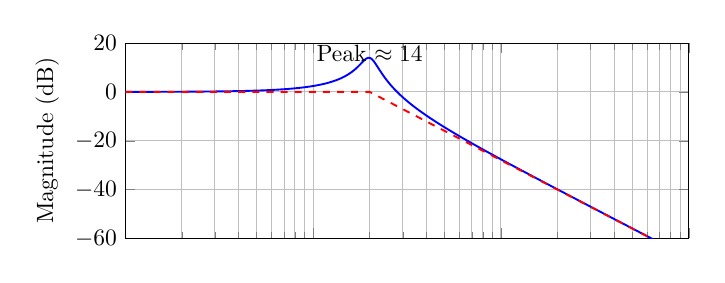
\begin{tikzpicture}[scale=0.85]
    \begin{semilogxaxis}[
        width=10cm, height=4.5cm,
        ylabel={Magnitude (dB)},
        xmin=1, xmax=1000,
        ymin=-60, ymax=20,
        grid=both,
        xtick={1,10,100,1000},
        xticklabels={},
        ytick={-60,-40,-20,0,20}
    ]
    \addplot[blue,thick,domain=1:1000,samples=300]
        {20*log10(400/sqrt((400-x^2)^2 + (4*x)^2))};
    \addplot[red,dashed,thick] coordinates {(1,0) (20,0) (1000,-68)};
    \node at (axis cs:20,16) {Peak $\approx 14\dB$};
    \end{semilogxaxis}
\end{tikzpicture}

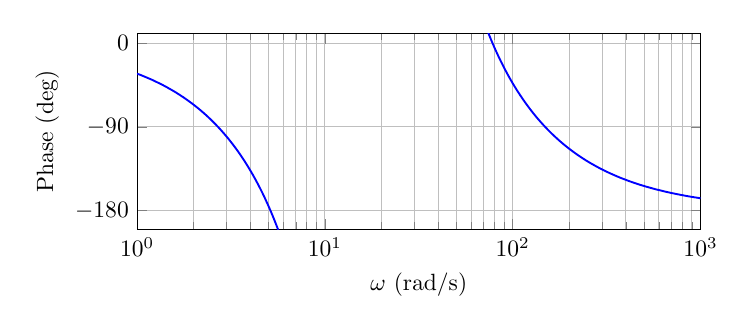
\begin{tikzpicture}[scale=0.85]
    \begin{semilogxaxis}[
        width=10cm, height=4.5cm,
        xlabel={$\omega$ (rad/s)},
        ylabel={Phase (deg)},
        xmin=1, xmax=1000,
        ymin=-200, ymax=10,
        grid=both,
        xtick={1,10,100,1000},
        ytick={-180,-90,0}
    ]
    \addplot[blue,thick,domain=1:19.9,samples=100]
        {-atan(4*x/(400-x^2))*180/pi};
    \addplot[blue,thick,domain=20.1:1000,samples=100]
        {-180-atan(4*x/(400-x^2))*180/pi};
    \end{semilogxaxis}
\end{tikzpicture}
\end{center}
\end{example}

\begin{example}[Transfer Function from Bode Plot]
\label{ex:identify}
The following Bode magnitude plot was measured experimentally. Determine the transfer function.

\begin{center}
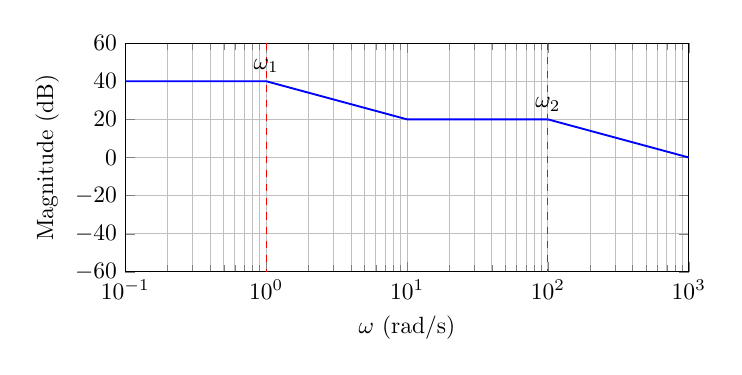
\begin{tikzpicture}[scale=0.85]
    \begin{semilogxaxis}[
        width=10cm, height=5cm,
        xlabel={$\omega$ (rad/s)},
        ylabel={Magnitude (dB)},
        xmin=0.1, xmax=1000,
        ymin=-60, ymax=60,
        grid=both,
        xtick={0.1,1,10,100,1000},
        ytick={-60,-40,-20,0,20,40,60}
    ]
    % Plot with specific characteristics
    \addplot[blue,thick] coordinates {
        (0.1,40) (1,40) (10,20) (100,20) (1000,0)
    };
    % Corner frequency markers
    \draw[dashed,red] (axis cs:1,60) -- (axis cs:1,-60);
    \draw[dashed,red] (axis cs:100,60) -- (axis cs:100,-60);
    \node[above] at (axis cs:1,40) {$\omega_1$};
    \node[above] at (axis cs:100,20) {$\omega_2$};
    \end{semilogxaxis}
\end{tikzpicture}
\end{center}

\textbf{Solution:}

\textit{Step 1: Identify corner frequencies.}
Initially, we observe a corner at $\omega_1 = 1$ rad/s where the slope changes from $0$ to $-20\dB$/decade, suggesting a pole. At $\omega_2 = 100$ rad/s, the slope changes again.

Wait---looking more carefully at the slope transitions: from $\omega = 0.1$ to $\omega = 1$, the slope is $0\dB$/decade; from $\omega = 1$ to $\omega = 10$, the slope is $(20-40)/(1) = -20\dB$/decade; from $\omega = 10$ to $\omega = 100$, the slope returns to $0\dB$/decade; and from $\omega = 100$ to $\omega = 1000$, the slope is again $-20\dB$/decade.

\textit{Step 2: Identify poles and zeros.}
At $\omega = 1$, the slope goes from $0$ to $-20$, indicating a \textbf{pole at $s = -1$}. At $\omega = 10$, the slope goes from $-20$ to $0$, indicating a \textbf{zero at $s = -10$}. At $\omega = 100$, the slope goes from $0$ to $-20$, indicating a \textbf{pole at $s = -100$}.

\textit{Step 3: Determine DC gain.}
At $\omega = 0.1$, magnitude $= 40\dB$. Extrapolating the low-frequency asymptote to $\omega = 1$:
\begin{equation}
K_0 = 10^{40/20} = 100
\end{equation}

\textit{Step 4: Construct transfer function.}
\begin{equation}
G(s) = 100 \cdot \frac{1 + s/10}{(1 + s)(1 + s/100)} = \frac{100(s + 10)}{(s + 1)(s + 100)}
\end{equation}

Verify: This can be simplified to check DC gain:
\begin{equation}
G(0) = \frac{100 \times 10}{1 \times 100} = 10 \Rightarrow 20\dB
\end{equation}

Hmm, this doesn't match our $40\dB$ reading. Let's reconsider.

\textit{Corrected Step 3:}
At very low frequency (below the first pole), the gain is $40\dB = 100$. The transfer function in standard form is:
\begin{equation}
G(s) = K \cdot \frac{(1 + s/10)}{(1 + s)(1 + s/100)}
\end{equation}

For DC gain of 100:
\begin{equation}
G(0) = K = 100 \checkmark
\end{equation}

Therefore:
\begin{equation}
\boxed{G(s) = \frac{100(1 + s/10)}{(1 + s)(1 + s/100)} = \frac{1000(s + 10)}{(s + 1)(s + 100)}}
\end{equation}
\end{example}

\begin{examplebox}[Finding Stability Margins]
\label{ex:margins}
For the open-loop transfer function $G(s) = \dfrac{100}{s(s+1)(s+10)}$, find the gain margin and phase margin.

\textbf{Solution:}

\textit{Step 1: Find the phase crossover frequency.}
At phase crossover, $\phase{G(\jw_{pc})} = -180\degrees$.

\begin{equation}
\phase{G(\jw)} = -90\degrees - \arctan(\omega) - \arctan(\omega/10)
\end{equation}

Setting this equal to $-180\degrees$:
\begin{equation}
-90\degrees - \arctan(\omega_{pc}) - \arctan(\omega_{pc}/10) = -180\degrees
\end{equation}
\begin{equation}
\arctan(\omega_{pc}) + \arctan(\omega_{pc}/10) = 90\degrees
\end{equation}

Using the identity $\arctan(a) + \arctan(b) = 90\degrees$ when $ab = 1$:
\begin{equation}
\omega_{pc} \cdot (\omega_{pc}/10) = 1 \Rightarrow \omega_{pc}^2 = 10 \Rightarrow \omega_{pc} = \sqrt{10} \approx 3.16 \text{ rad/s}
\end{equation}

\textit{Step 2: Calculate gain margin.}
\begin{equation}
\magn{G(j\sqrt{10})} = \frac{100}{\sqrt{10} \cdot \sqrt{1+10} \cdot \sqrt{1+0.1}} = \frac{100}{\sqrt{10} \cdot \sqrt{11} \cdot \sqrt{1.1}}
\end{equation}
\begin{equation}
= \frac{100}{\sqrt{121}} = \frac{100}{11} \approx 9.09
\end{equation}

\begin{equation}
\text{GM} = \frac{1}{9.09} = 0.11 \Rightarrow \text{GM}_{\text{dB}} = 20\log_{10}(0.11) = -19.2\dB
\end{equation}

Since the gain at phase crossover is greater than 1, the gain margin is \textbf{negative}, indicating an \textbf{unstable} closed-loop system!

\textit{Step 3: Find the gain crossover frequency.}
We need $\magn{G(\jw_{gc})} = 1$:
\begin{equation}
\frac{100}{\omega_{gc}\sqrt{1+\omega_{gc}^2}\sqrt{1+\omega_{gc}^2/100}} = 1
\end{equation}

This requires numerical solution. Testing $\omega_{gc} = 4.3$:
\begin{equation}
\frac{100}{4.3 \cdot \sqrt{1+18.49} \cdot \sqrt{1+0.185}} = \frac{100}{4.3 \cdot 4.41 \cdot 1.09} \approx 4.8 \neq 1
\end{equation}

Testing $\omega_{gc} = 8$:
\begin{equation}
\frac{100}{8 \cdot \sqrt{65} \cdot \sqrt{1.64}} = \frac{100}{8 \cdot 8.06 \cdot 1.28} \approx 1.21
\end{equation}

Testing $\omega_{gc} = 9$:
\begin{equation}
\frac{100}{9 \cdot \sqrt{82} \cdot \sqrt{1.81}} = \frac{100}{9 \cdot 9.06 \cdot 1.35} \approx 0.91
\end{equation}

By interpolation, $\omega_{gc} \approx 8.5$ rad/s.

\textit{Step 4: Calculate phase margin.}
\begin{equation}
\phase{G(j8.5)} = -90\degrees - \arctan(8.5) - \arctan(0.85)
\end{equation}
\begin{equation}
= -90\degrees - 83.3\degrees - 40.4\degrees = -213.7\degrees
\end{equation}

\begin{equation}
\text{PM} = 180\degrees + (-213.7\degrees) = -33.7\degrees
\end{equation}

The \textbf{negative phase margin} confirms instability.

\textit{Conclusion:} The closed-loop system with unity feedback is \textbf{unstable}. Both gain margin and phase margin are negative.
\end{examplebox}

\begin{example}[Designing for Specified Bandwidth]
\label{ex:bandwidth}
A unity feedback system has open-loop transfer function $G(s) = \dfrac{K}{s(s+5)}$. Determine the value of $K$ that gives a closed-loop bandwidth of $10$ rad/s.

\textbf{Solution:}

The closed-loop transfer function is:
\begin{equation}
T(s) = \frac{G(s)}{1+G(s)} = \frac{K}{s^2 + 5s + K}
\end{equation}

Comparing with the standard second-order form:
\begin{equation}
T(s) = \frac{\omega_n^2}{s^2 + 2\zeta\omega_n s + \omega_n^2}
\end{equation}

We identify:
\begin{align}
\omega_n^2 &= K \Rightarrow \omega_n = \sqrt{K} \\
2\zeta\omega_n &= 5 \Rightarrow \zeta = \frac{5}{2\sqrt{K}}
\end{align}

The bandwidth of a second-order system is approximately:
\begin{equation}
\omega_{BW} \approx \omega_n\sqrt{1 - 2\zeta^2 + \sqrt{4\zeta^4 - 4\zeta^2 + 2}}
\end{equation}

For moderate damping ($\zeta \approx 0.5$ to $0.7$), a useful approximation is $\omega_{BW} \approx \omega_n$ to $1.5\omega_n$.

Setting $\omega_{BW} = 10$ rad/s and using $\omega_{BW} \approx \omega_n$ as a first estimate:
\begin{equation}
\omega_n = 10 \Rightarrow K = 100
\end{equation}

Check the damping ratio:
\begin{equation}
\zeta = \frac{5}{2\sqrt{100}} = \frac{5}{20} = 0.25
\end{equation}

This is underdamped. The exact bandwidth formula gives:
\begin{equation}
\omega_{BW} = 10\sqrt{1 - 0.125 + \sqrt{0.0039 - 0.25 + 2}} = 10\sqrt{0.875 + 1.32} = 10 \times 1.48 = 14.8 \text{ rad/s}
\end{equation}

This overshoots our target. Iterate with lower $K$:

Try $K = 50$: $\omega_n = 7.07$, $\zeta = 0.354$
\begin{equation}
\omega_{BW} = 7.07\sqrt{0.75 + 1.19} = 7.07 \times 1.39 = 9.8 \text{ rad/s} \approx 10 \text{ rad/s} \checkmark
\end{equation}

\textit{Final Answer:} $\boxed{K \approx 50}$
\end{example}

\begin{example}[Complete Bode Plot with Multiple Elements]
\label{ex:complete}
Sketch the Bode plot for:
\begin{equation}
G(s) = \frac{1000(s+10)}{s(s+1)(s+100)}
\end{equation}

\textbf{Solution:}

\textit{Step 1: Rewrite in standard form.}
\begin{equation}
G(s) = \frac{1000 \cdot 10 \cdot (1 + s/10)}{s \cdot 1 \cdot (1+s) \cdot 100 \cdot (1+s/100)} = \frac{100(1+s/10)}{s(1+s)(1+s/100)}
\end{equation}

\textit{Step 2: Identify components.}

\begin{center}
\begin{tabular}{lll}
\toprule
Element & Corner (rad/s) & Contribution \\
\midrule
Gain $K = 100$ & -- & $+40\dB$ \\
Pole at origin & -- & $-20\dB$/dec, $-90\degrees$ \\
Pole at $s = -1$ & $\omega = 1$ & $-20\dB$/dec, $-90\degrees$ \\
Zero at $s = -10$ & $\omega = 10$ & $+20\dB$/dec, $+90\degrees$ \\
Pole at $s = -100$ & $\omega = 100$ & $-20\dB$/dec, $-90\degrees$ \\
\bottomrule
\end{tabular}
\end{center}

\textit{Step 3: Construct magnitude asymptotes.}

At $\omega = 1$ (before any corners except pole at origin):
\begin{equation}
\magn{G(j \cdot 1)}_{\text{dB}} \approx 40\dB - 20\log_{10}(1) = 40\dB
\end{equation}

The asymptotic slopes vary with frequency: for $\omega < 1$, the slope is $-20\dB$/dec; for $1 < \omega < 10$, the slope steepens to $-40\dB$/dec; for $10 < \omega < 100$, the slope returns to $-20\dB$/dec; and for $\omega > 100$, the slope is again $-40\dB$/dec.

\textit{Step 4: Construct phase.}
\begin{equation}
\phase{G(\jw)} = -90\degrees - \arctan(\omega) + \arctan(\omega/10) - \arctan(\omega/100)
\end{equation}

Key phase values are computed as follows: as $\omega \to 0$, $\phase{G} \to -90\degrees$; at $\omega = 1$, $\phase{G} = -90 - 45 + 5.7 - 0.6 = -130\degrees$; at $\omega = 10$, $\phase{G} = -90 - 84.3 + 45 - 5.7 = -135\degrees$; at $\omega = 100$, $\phase{G} = -90 - 89.4 + 84.3 - 45 = -140\degrees$; and as $\omega \to \infty$, $\phase{G} \to -90 - 90 + 90 - 90 = -180\degrees$.

\begin{center}
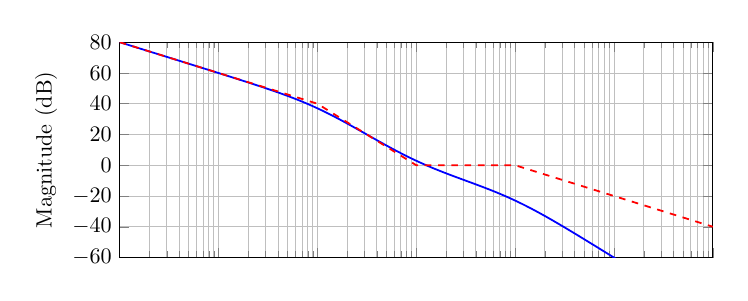
\begin{tikzpicture}[scale=0.8]
    \begin{semilogxaxis}[
        width=11cm, height=5cm,
        ylabel={Magnitude (dB)},
        xmin=0.01, xmax=10000,
        ymin=-60, ymax=80,
        grid=both,
        xtick={0.01,0.1,1,10,100,1000,10000},
        xticklabels={},
        ytick={-60,-40,-20,0,20,40,60,80}
    ]
    % Exact magnitude
    \addplot[blue,thick,domain=0.01:10000,samples=300]
        {40 + 20*log10(sqrt(1+(x/10)^2)) - 20*log10(x) - 20*log10(sqrt(1+x^2)) - 20*log10(sqrt(1+(x/100)^2))};

    % Asymptotes
    \addplot[red,dashed,thick] coordinates {
        (0.01,80) (1,40) (10,0) (100,0) (10000,-40)
    };
    \end{semilogxaxis}
\end{tikzpicture}

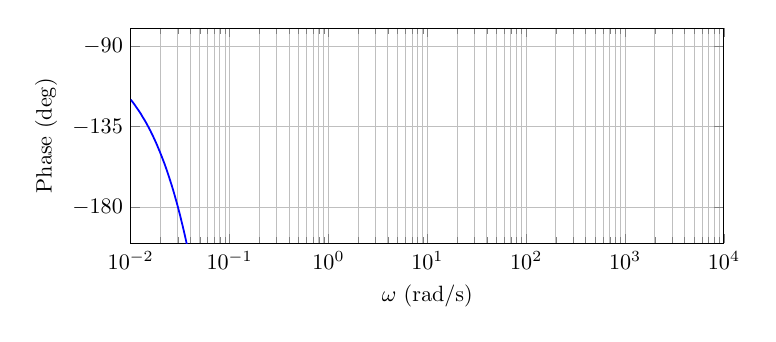
\begin{tikzpicture}[scale=0.8]
    \begin{semilogxaxis}[
        width=11cm, height=5cm,
        xlabel={$\omega$ (rad/s)},
        ylabel={Phase (deg)},
        xmin=0.01, xmax=10000,
        ymin=-200, ymax=-80,
        grid=both,
        xtick={0.01,0.1,1,10,100,1000,10000},
        ytick={-180,-135,-90}
    ]
    % Exact phase
    \addplot[blue,thick,domain=0.01:10000,samples=300]
        {-90 - atan(x)*180/pi + atan(x/10)*180/pi - atan(x/100)*180/pi};
    \end{semilogxaxis}
\end{tikzpicture}
\end{center}
\end{example}

%=============================================================================
\section{Summary}
\label{sec:summary}
%=============================================================================

This chapter has introduced the frequency response method---a powerful technique for analyzing and designing control systems without solving differential equations.

The \textbf{frequency response}, obtained by evaluating the transfer function along the imaginary axis as $G(\jw)$, completely characterizes the steady-state response to sinusoidal inputs. \textbf{Bode plots}---logarithmic plots of magnitude (in dB) and phase (in degrees) versus frequency---enable graphical analysis of complex systems through superposition. The \textbf{asymptotic approximations} that make Bode plots practical follow simple rules: first-order terms contribute $\pm 20\dB$/decade and $\pm 90\degrees$ per pole or zero, while second-order terms contribute $\pm 40\dB$/decade and $\pm 180\degrees$. \textbf{Stability margins}, specifically gain margin (how much gain can increase) and phase margin (how much phase can lag), quantify robustness and are read directly from the Bode plot. Finally, from a \textbf{practical application} standpoint, the frequency response can be measured experimentally, enabling system identification and verification of theoretical models.

\begin{keypoint}
The frequency response method transforms the complexity of differential equations into intuitive graphical reasoning. This approach, pioneered at Bell Labs in the 1930s and 1940s, remains the foundation of practical control system design.
\end{keypoint}

%=============================================================================
\newpage
\section{Exercises}
\label{sec:exercises}
%=============================================================================

\begin{exercise}
Sketch the Bode plot for $G(s) = \dfrac{50}{(s+5)(s+50)}$. Determine the corner frequencies and the DC gain.
\end{exercise}

\begin{exercise}
For the transfer function $G(s) = \dfrac{s+2}{s^2+3s+2}$, sketch the Bode plot and identify any pole-zero cancellations.
\end{exercise}

\begin{exercise}
A system has the open-loop transfer function $G(s) = \dfrac{K}{s(s+2)(s+8)}$. Find the range of $K$ for closed-loop stability using the Bode plot method.
\end{exercise}

\begin{exercise}
From the following measured data, estimate the transfer function:
\begin{center}
\begin{tabular}{ccc}
\toprule
$\omega$ (rad/s) & Magnitude (dB) & Phase (degrees) \\
\midrule
0.1 & 20 & $-6\degrees$ \\
1 & 17 & $-45\degrees$ \\
10 & $-3$ & $-84\degrees$ \\
100 & $-23$ & $-90\degrees$ \\
\bottomrule
\end{tabular}
\end{center}
\end{exercise}

\begin{exercise}
A second-order system has $\omega_n = 50$ rad/s and $\zeta = 0.2$. Calculate the resonant peak magnitude and the frequency at which it occurs.
\end{exercise}

\begin{exercise}
Design a lead compensator $G_c(s) = K\dfrac{s+a}{s+b}$ (with $b > a$) to provide $45\degrees$ of phase lead at $\omega = 10$ rad/s.
\end{exercise}

\begin{exercise}
An RC filter with $R = 1\,\text{k}\Omega$ is to have a corner frequency of $1\,\text{kHz}$. Calculate the required capacitor value and sketch the expected Bode plot.
\end{exercise}

\begin{exercise}
For a unity feedback system with $G(s) = \dfrac{100(s+1)}{s^2(s+10)}$, find the gain margin and phase margin. Is the system stable?
\end{exercise}

\begin{exercise}
Explain why a phase margin of $45\degrees$ to $60\degrees$ is typically specified in control system design. What happens if the phase margin is too small? Too large?
\end{exercise}

\begin{exercise}
Using an Arduino or similar microcontroller, design an experiment to measure the frequency response of a simple audio amplifier circuit. Specify the frequency range, number of test points, and expected measurement accuracy.
\end{exercise}

\begin{exercise}
For the transfer function $G(s) = \dfrac{10(s+2)}{s(s+1)(s+20)}$, construct the Bode magnitude and phase plots using asymptotic approximations. Identify all corner frequencies and the slopes of each asymptotic region.
\end{exercise}

\begin{exercise}
A control system has open-loop transfer function $G(s) = \dfrac{K(s+5)}{s^2(s+50)}$. Determine the value of $K$ that provides a phase margin of exactly $45\degrees$. What is the corresponding gain margin?
\end{exercise}

%=============================================================================
% Bibliography would go here in a full textbook
%=============================================================================

\section*{Further Reading}

For those seeking deeper understanding, several classic and modern references are recommended. Bode's own work, \textit{Network Analysis and Feedback Amplifier Design} (Van Nostrand, 1945), remains the definitive classic reference on frequency response methods. Nyquist's foundational 1932 paper ``Regeneration Theory'' in the \textit{Bell System Technical Journal} (Vol.\ 11, No.\ 1, pp.\ 126--147) established the theoretical basis for stability analysis using frequency response. Among modern textbooks, Franklin, Powell, and Emami-Naeini's \textit{Feedback Control of Dynamic Systems} (8th ed., Pearson, 2019) provides excellent coverage with MATLAB examples. Ogata's \textit{Modern Control Engineering} (5th ed., Prentice Hall, 2010) offers comprehensive coverage of both classical and modern methods. Dorf and Bishop's \textit{Modern Control Systems} (13th ed., Pearson, 2017) is particularly noted for its excellent problems and applications.

